To validate the feasibility of the proposed control structure, the individual controllers are tested independently, and the full cascaded structure is then tested in concert. The small-signal model is used for all simulation tests; while this is inherently less accurate than testing against the full nonlinear model \cref{eq:NonLinearModelWithTank}, this model's stiffness requires a sampling interval that, considering the computational complexity of each timestep and the timescale of the dynamics, is impracticable.

We first present results pertaining to the VFLQR under the assumption that disturbances are perfectly known, and that the exact flows demanded are delivered by the inner loop. The controller is tested against nominal conditions, as well as a variety of non-nominal conditions - respectively $50\%$ slower and $200\%$ faster true dynamics than the nominal model, and against a constant output disturbance\footnote{Equivalent to e.g. a small leak in the pressure vessel.} of $-0.1 \frac{\si{bar}}{100\si{s}}$. We note that in each case the controls are clamped to $\{0, 3.5\} \frac{\si{m^3}}{\si{hr}}$ corresponding to the provided pump curves \cite{GrundfosDatablad}, and the system is subjected to a slowly time-varying state disturbance. The results can be seen on \cref{fig:LQRTracking}, displaying tracking performance in each case that is excellent; the disturbance is completely rejected, and the system converges to and maintains the reference. 


\begin{figure}[h!]
	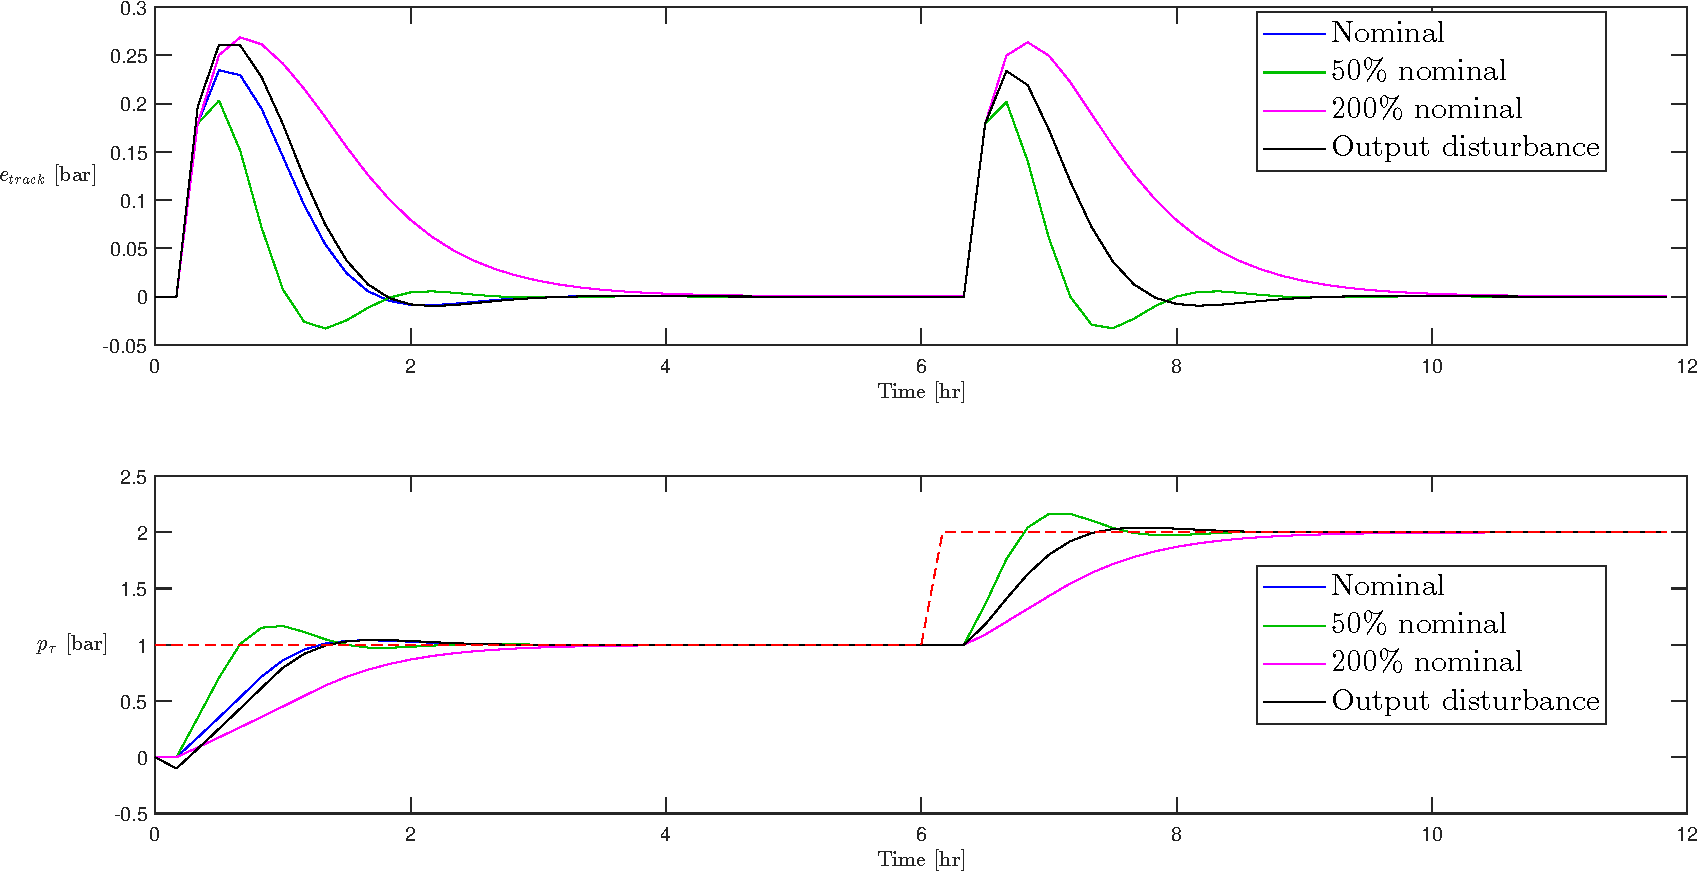
\includegraphics[height=4cm, width=\linewidth]{Graphics/LQRTracking.pdf}
	\caption{Outer loop simulation}
	\label{fig:LQRTracking}
\end{figure}

 We now examine the behaviour of the inner loop under two separate step references. Note that these references represent deviations from the equilibrium flows. The PID controllers are limited to the range $\{-66,34\}$, corresponding to the inputs $\{0,100\}$ to the full system, with a back-calculation anti-windup scheme.

\begin{figure}[h!]
	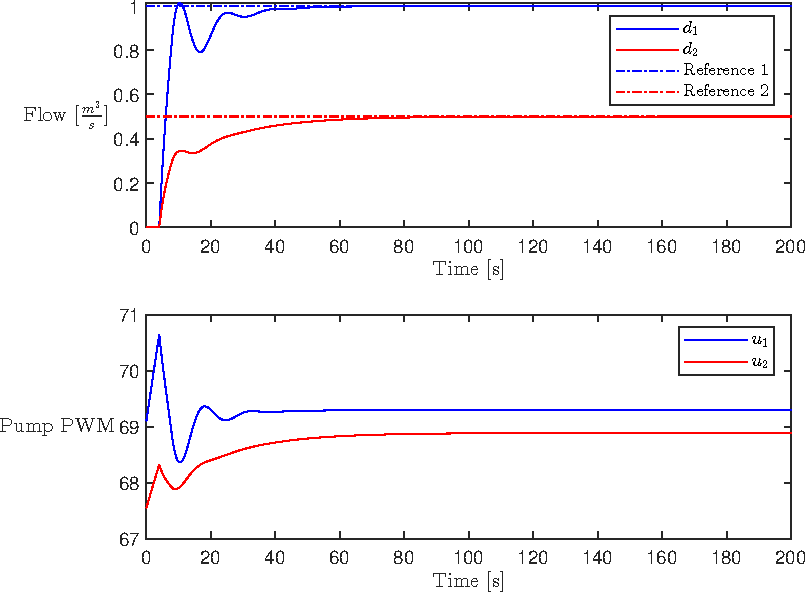
\includegraphics[width=\linewidth,height=4cm]{Graphics/PumpSimulation.pdf}
	\caption{Inner loop simulation}
	\label{fig:PumpSimulation}
\end{figure}

The results on \cref{fig:PumpSimulation} show a convergence speed of roughly $40 \si{s}$ and limited ringing as desired. The ringing displayed by $d_1$ can be limited by ramp-limiting reference changes from the outer loop, which should not cause issues as the outer loop is clearly significantly slower than the inner loop. Finally, we evaluate the full cascaded control structure, again under the influence of a time-varying (but perfectly measurable) disturbance.

\begin{figure}[h!]
	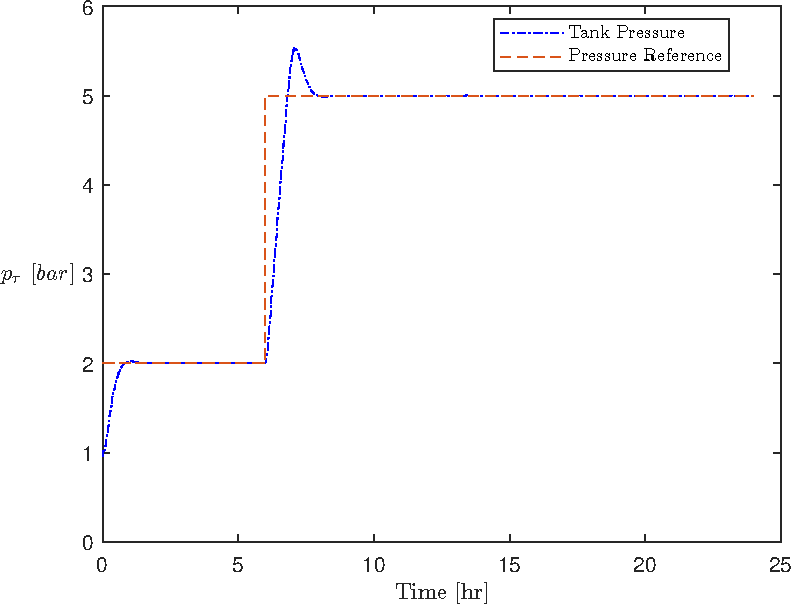
\includegraphics[height=4cm, width=\linewidth]{Graphics/FullSimPressures.pdf}
	\caption{Outer loop, cascaded simulation}
	\label{fig:FullSimPressure}
\end{figure}

\begin{figure}[h!]
	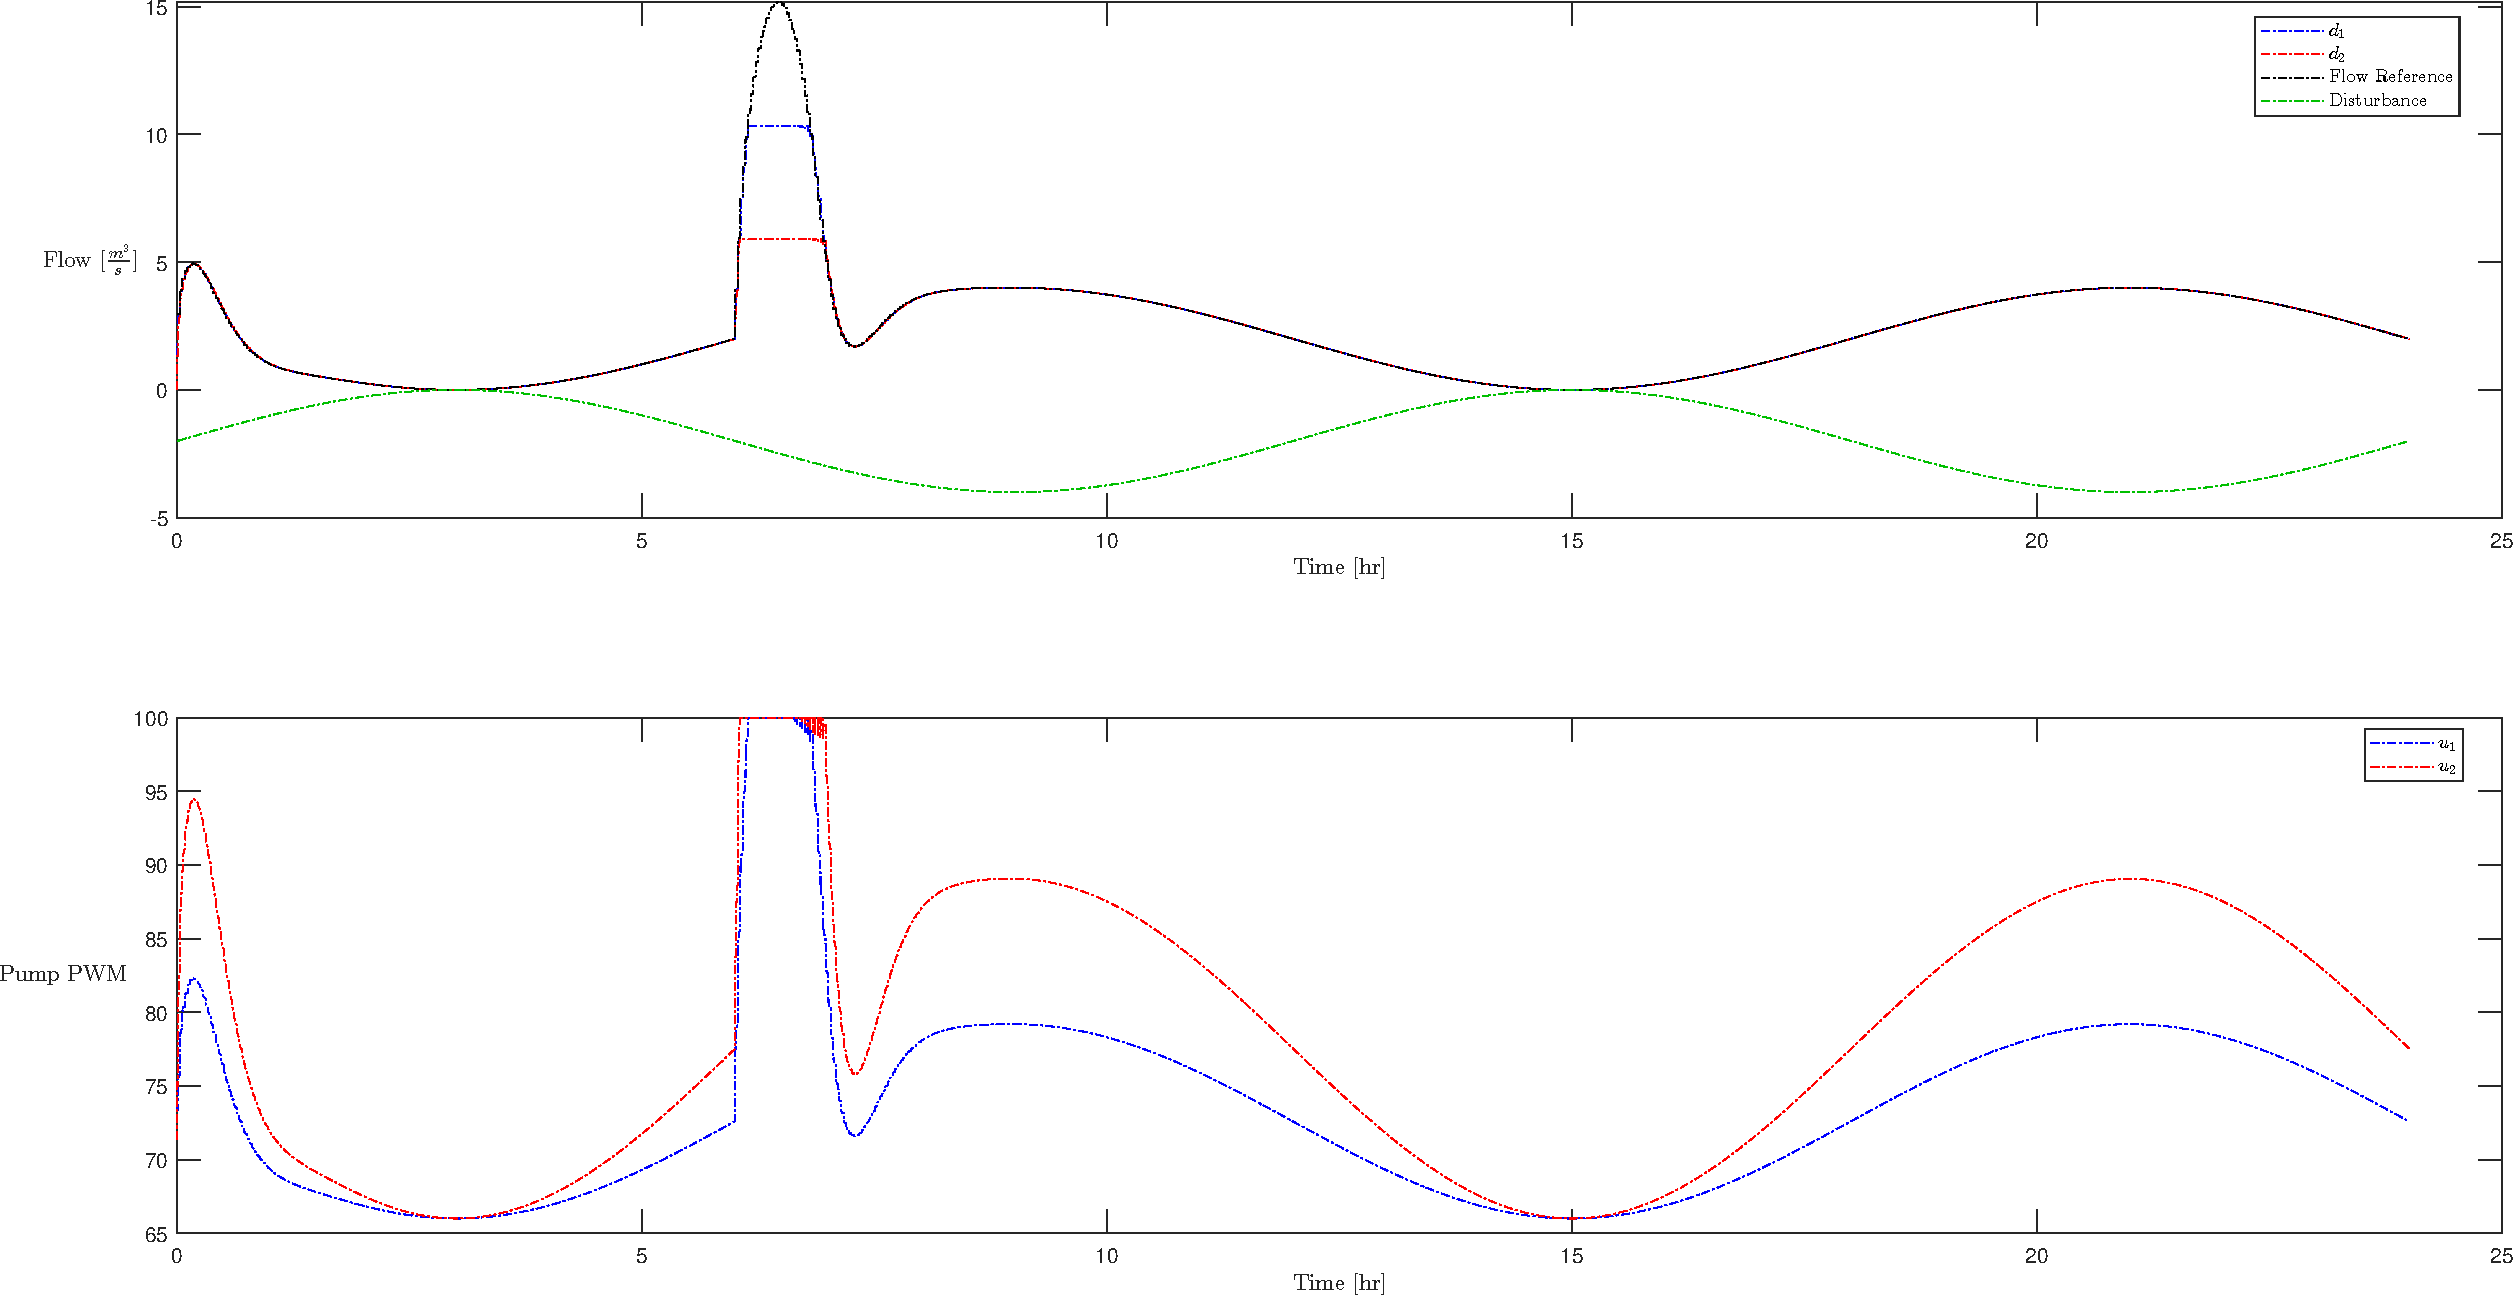
\includegraphics[height=4cm, width=\linewidth]{Graphics/FullSimFlows.pdf}
	\caption{Inner loop, cascaded simulation}
	\label{fig:FullSimFlows}
\end{figure}

We note, as before, offset-free tracking. There is some overshoot after the reference change from $p_{ref} = 2 \ \si{bar}$ to $p_{ref} = 5 \ \si{bar}$; this is caused by the clamping of the the pumps to their maximum operating speed when the desired flow reference from the outer loop becomes too large, as the outer loop does not have anti-windup functionality. We note additionally that, as expected, the outer loop compensates for the time-varying disturbance by sign-reversed injection of the disturbance as a control signal. In theory, this means that the outer loop can reject an arbitrary disturbance - as opposed to e.g. only constant or integrating disturbances - so long as it is measurable or estimateable. Furthermore, the steady-state error is bounded from below by the disturbance estimate error insofar as rejecting the disturbance does not saturate any actuators.




